\documentclass[conference]{IEEEtran}
\IEEEoverridecommandlockouts
% The preceding line is only needed to identify funding in the first footnote. If that is unneeded, please comment it out.
\usepackage{cite}
\usepackage{amsmath,amssymb,amsfonts}
\usepackage{algorithmic}
\usepackage{graphicx}
\usepackage{textcomp}
\usepackage{adjustbox} 
\usepackage{xcolor}
\usepackage{float}
\usepackage{hyperref}
\usepackage{placeins}
\def\BibTeX{{\rm B\kern-.05em{\sc i\kern-.025em b}\kern-.08em
    T\kern-.1667em\lower.7ex\hbox{E}\kern-.125emX}}
\hypersetup{
    colorlinks=true,
    linkcolor=black,
    citecolor=black,
    filecolor=black,
    urlcolor=blue,  
}
\begin{document}
\title{Eye Disease Detection using Convolutional Neural Networks\\
\vspace{10pt}
\fontsize{12}{14}\selectfont GitHub Repo Link: \href{https://github.com/VishanthSurresh/COMP478-Image_Processing_Project-Eye_Disease_Classification/blob/main/CNN\%20Model/eye-disease-classification.ipynb}{https://github.com/EyeDiseaseDetection}
}




\author{\IEEEauthorblockN{1\textsuperscript{st} Vishanth Surresh - 40181942}
\IEEEauthorblockA{\textit{Department of Computer Science and Engineering} \\
\textit{Concordia University}\\
Montreal, Canada \\
\textit{v\_surres\char`\@live.concordia.ca} }
\and
\IEEEauthorblockN{2\textsuperscript{nd} Rajat Kumar - 40201807}
\IEEEauthorblockA{\textit{Department of Software Engineering} \\
\textit{Concordia University}\\
Montreal, Canada \\
rajat.kumar@mail.concordia.ca}
}
\maketitle

\begin{abstract}
Eye diseases can significantly affect a person’s vision and quality of life. Eye diseases continue to rise, this increase can be linked to the factor like increase in screen time, unhealthy lifestyle, exposure to radiations and other health issues like diabetics. Some of the common eye diseases include Diabetic Retinopathy, Cataract and Glaucoma. As per WHO cataract is one of the major causes for blindness and visual impairment in the world. However, if these diseases are detected at an early stage they can be treated. Deep Learning techniques has shown great potential in detecting such diseases. In this study we use propose a deep learning approach based on a Convolutional Neural Network (CNN) architecture, to detect diabetic retinopathy, cataract, and glaucoma. The dataset comprises of 4217 retinal images which is divided into train and test sets. To ensure robustness and to prevent over fitting, the dataset is trained using K-Fold cross-validation. We have used accuracy, precision, recall, and F1-score to evaluate the performance of our model. 
\end{abstract}
\begin{IEEEkeywords}
CNN, Deep Learning, Image Classification, Image Processing, Medical Image Analysis
\end{IEEEkeywords}

\section{Introduction}
Vision is one of the most important parts of a person’s life, all day-to-day important tasks we perform need a healthy vision to execute them. With increase in screen times, unhealthy lifestyle and increase in life expectancy, eye diseases are becoming increasingly prevalent and a leading cause for blindness. However, if these diseases are detected at an early stage, then then we can prevent them from causing serious conditions like loss of vision and even blindness. If neglected, most of these eye diseases can lead to irreversible vision loss. Early-stage, detection of such diseases and then treatment for it can aid in slowed or halted disease progression, conserving eyesight and lowering the chance of blindness. For example, currently there is no cure for glaucoma, but an early diagnosis can limit the vision loss using medications or surgery.

\vspace{5pt}
Typically, to detect such diseases ophthalmologists inspect the patient’s eyes and evaluate the retinal pictures for any indications of any abnormalities. This procedure is quite time consuming, costly and requires an ophthalmologist to examine the patient’s eye. With eye diseases increasing rapidly, it may not be possible for doctors to instantly attend the patient and give the diagnosis. Also, not all people can afford such costly procedures.

\vspace{5pt} 
Deep learning techniques have shown promising ability in detecting these diseases using image classification techniques. With the power of Artificial Intelligence (AI) and machine learning, deep learning models are trained to process complex retinal images and detect various eyes diseases like diabetic retinopathy, cataract, and glaucoma with remarkable precision.In deep learning, a computer model learns to performs classification tasks directly from images. The accuracy obtained by deep learning models have shown the potential of exceeding human-level accuracy. Deep learning models are trained using a large set of labeled data and neural network architectures that contain multiple layers. Deep learning models are also known as deep neural networks as they use neural network architectures. Deep Learning applications are used in various industries such as Automated Driving, Aerospace and Defense, Medical Research, industrial Automation and Electronics. However, this paper focuses only on how deep learning technologies can be used for timely detection of various eye diseases like Diabetic Retinopathy, Cataract and Glaucoma. 

\vspace{5pt}
One such deep learning algorithm which has shown the most promising results in this field is Convolutional Neural Networks (CNN's). CNN has shown good success in fields such as object recognition, facial recognition, and medical image analysis. Hence, there is a lot of potential in using CNN's for automating the process of classification analysis of retinal images to ensure early detection of eye diseases.

\vspace{5pt}
Convolutional Neural Networks (CNNs) are well suited for processing 2D data such as images as they use 2D convolution layers. A typical CNN have two main parts, a convolution/pooling mechanism that breaks up the image into features and analyzes them and the other one is a fully connected layer that predicts the best label to classify the image by taking the output from the convolution/pooling layers.

\vspace{5pt}
A typical image classification process consists of an input which is a set of N images, each labeled with one of K different classes. This data is called the training set Fig[\ref{fig 1:Image Classification Pipeline}]. This data is used to learn what each of the classes look like and this step is known as training a classifier or learning a model. In the last step we assess the quality of our classifier by asking it to predict levels for a new set of images which we call as the test set. The true labels of these images are compared with the labels predicted by our model to check the accuracy and precision of our model. More correct predictions mean better accuracy and precision for the model.

\begin{figure}[ht]
    \centering
    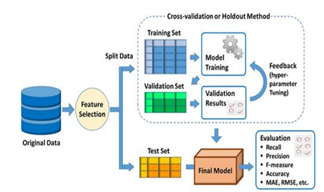
\includegraphics[width=9cm, height = 5cm]{Images/Architecture.png}
    \caption{Image Classification Pipeline}
    \label{fig 1:Image Classification Pipeline}
\end{figure}

\vspace{5pt}
This report gives an overview about how we developed the Image classification model using CNN that helps to detect various eye disease like diabetic retinopathy, cataract and glaucoma. Main aim of our study is to develop an Image classification model which can successfully provide an early detection of such diseases. By building this model we want to decrease the cost, time, reliance on human expertise and ensure a higher degree of accuracy while detecting eye diseases.

\vspace{5pt}
The report is divided into the following sections. First section talks about the related work in this field, that is using CNN models for classification of eye diseases. In the second section we talk about the dataset that is being used for this study consisting of retinal images labeled into four categories namely Normal, Diabetic Retinopathy, Cataract, and Glaucoma. In the third section we talk about the prepossessing steps that we implement to ensure our dataset is compatible with the CNN model. In the fourth section we describe the CNN model architecture, activation functions and optimization techniques used for image classification. Lastly we present our findings on performance metrics such as accuracy, loss, precision, recall, and F1-score and conclusion on how our image classification model fairs in detecting eye diseases.

\section{Related Work}
A lot of research has been done in using image processing techniques to detect eye related abnormalities. Some of the early works include research by Abràmoff et al. (2013) \cite{b7}, which used colored retinal images as the data set to train their deep learning algorithm. The results of the study showed that the algorithm can be used to detect eye diseases such as diabetic retinopathy. 

\vspace{5pt}
Study conducted by Oluwatobi Noah Akande \cite{b8} used framework with two different approaches for retina image recognition. For healthy retinal image recognition, the first method used structural features; for DR retinal image recognition, the second method used vascular and lesion-based features. The results of the study showed Recognition rates of 100\% and 97.23\% for the healthy and DR retinal images, respectively, the results of the study also showed false acceptance rates of 0.0444 and a false rejection rate of 0.0133.

\vspace{5pt}
Another study conducted on detecting Diabetic eye diseases using Image Processing proposed a Diabetic Eye Disease (DED) classification framework based on a newly build convolution neural network. The newly developed CNN in this study combined with the traditional image processing displayed best performance accuracy for DED classification problems. The accuracy, specify and sensitivity results obtained from this model were also adequate. The study also compared the results obtained from the newly build CNN model with the three existing pre trained deep learning models Xception, VGG16, and DenseNet21.\cite{b9}

\vspace{5pt}
One of the recent study conducted by Farrikh Alzami \cite{b10} utilized fractal dimension as one of the extracted features to distinguish the healthy subjects and diabetic retinopathy patients. The study used MESSIDOR dataset and Random Forest as Classifier to obtain results that detect diabetic retinopathy in patients. Also the results of the study suggested to explore other features such as univariate, multivariate, other statistical features and red lesion detection to gain more information about diabetic retinopathy grade level.

\vspace{5pt}
A study conducted by Yogesh Kumar \cite{b11} aimed to predict various eye diseases, including Glaucoma, Cataract, Choroidal Neovascularization, Diabetic Macular Edema, and DRUSEN, using several convolutional neural network architectures. Basic CNN, Deep CNN, AlexNet 2, Xception, Inception V3, ResNet 50, and DenseNet121 were used in the study. The simulation results revealed that ResNet50 beat all other methods and achieved a validation accuracy of 98.9\%. Additionally, the Xception model performed well and had an accuracy rate of 98.4\%. 

\vspace{5pt}
An interesting study conducted in the area of classification used three different kinds of classifiers: artificial neural network, fuzzy classifier and neuro-fuzzy classifier to classify three types of diseases Cataract, Iridocyclitis and Corneal Haze. The results of the study demonstrated that fuzzy and neuro-fuzzy classifiers, are superior than the neural network classifier as they both had a detection rate of more than 90\% for classification of normal, cataract and iridocyclitis images. Also, their sensitivity was 88\% higher than the neural network classifier. Also, these classifiers were run on a database of 135 subjects using cross-validation strategy.\cite{b12}

\vspace{5pt}
Another interesting study conducted by Moahmmed Rashid Ahmed used MATLAB Deep Convolutional Neural Network (DCNN). This system works like a human brain with input, neurons, hidden layers and output. The deep convolutional neural network used here consists of one hidden layer, 16 input neuron and 2 output either healthy or not. In this study the dataset was split into train and test dataset with 70\% for training 15\% validation and 15\% for testing. Accuracy of this model came out to 92.78\% with execution time of 5.33s which depends on the number of iterations and epochs. \cite{b13}

\vspace{5pt}
Lastly Jena developed a model based on fully convolutional neural network for the classification of diabetic retinopathy. The proposed neural network consisted of only six convolutional layers along rectified linear unit (ReLU) activation and max pooling layer. This model trained faster as compared to traditional convolution neural network models. “The intelligence of our model lies in its ability to re-tune weight to overcome outliers encountered in future. The proposed model works well with an accuracy of 91.66\%.” \cite{b14}


\section{Proposed Methodology}

\subsection{Dataset}\label{AA}
The dataset is from Kaggle and contains 4217 images \cite{b15}. The dataset consists of Normal, Diabetic Retinopathy, Cataract and Glaucoma retinal images where each class have approximately 1000 images Table[\ref{tab:Dataset Distribution}] Fig[\ref{fig:Sample Training Images}]. These images are collected from various sources like IDRiD, Oculur recognition, HRF etc.

\begin{table}[h]
\centering
\begin{adjustbox}{width= 5cm, height=1.3cm}
\begin{tabular}{|c|c|}
\hline
\textbf{Eye Disease Type} & \textbf{Number of Images} \\ \hline
Cataract & 1038 \\ \hline
Diabetic Retinopathy & 1098 \\ \hline
Glaucoma & 1007 \\ \hline
Normal & 1074 \\ \hline
\end{tabular}
\end{adjustbox}
\vspace{5pt}
\caption{Dataset Distribution}
\label{tab:Dataset Distribution}
\end{table}

\begin{figure*}[ht]
    \centering
    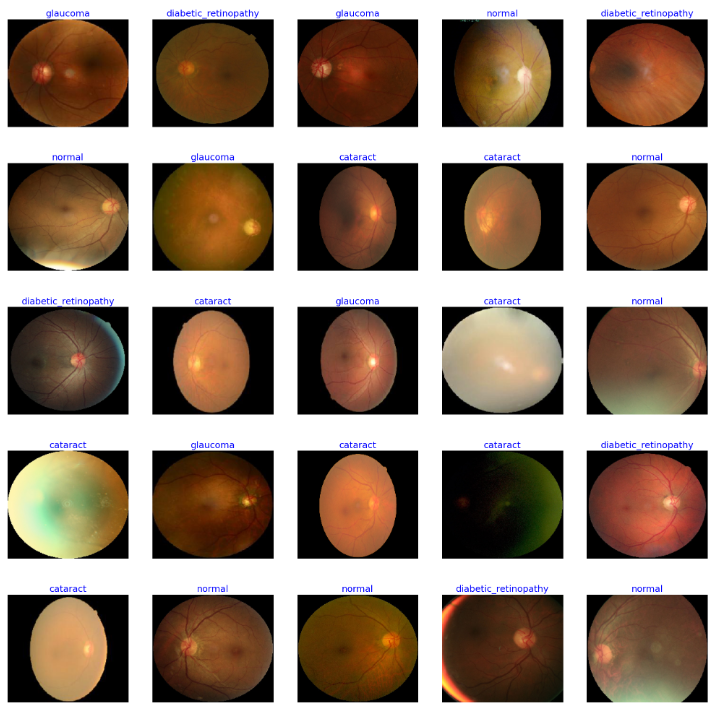
\includegraphics[width=0.8\textwidth,height = 11cm]{Images/Sample Images.png}
    \caption{Sample Training Images}
    \label{fig:Sample Training Images}
\end{figure*}


\subsection{Model architecture}
A convolution neural network consists of input layer, hidden layer and output layer Fig[\ref{fig:Sample Deep Learning  Architecture}]. Generally,  in feed forward network middle layers are referenced as hidden layers as their inputs and outputs are masked by activation function and final convolution. In this project we have used 4 convolution layers with input of [3 * 32 * 32]. The input is feed forwarded into the first convolution layer, where 3 is the number of channels i.e. RGB in our case and 32, 32 are the height and width of the image.

\vspace{5pt}
Each of these 4 convolution layers has the kernel size of (3,3), stride of (1,1) and padding of (1,1). The convolution layer is followed by a Batch Norm Layer which is used to distribute data uniformly across a mean that is best to the network. The batch normalization is followed by the Activation function. Here we used ReLU as the activation function. There are two pooling layers, each after every 2 convolution layers. Max pooling with a filter of (2,2) and a stride of 2 was used. Padding help to retain more information at the border of the image. The Dropout function is used to avoid over-fitting of the model. Finally output from final pooling layer is flattened and fed as an input to the fully connect layer. Neurons in fully connected layer was connected to activation's in previous layer which helps classify data into multiple classes.

\begin{figure}[ht]
    \centering
    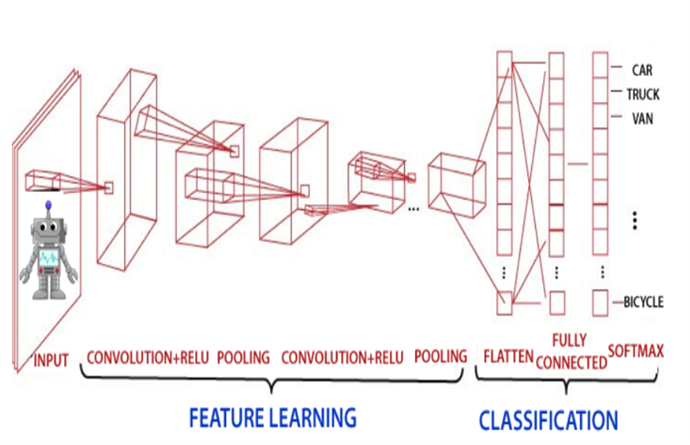
\includegraphics[width=9cm, height = 5cm]{Images/Deep Learning Architecture.png}
    \caption{Sample Deep Learning Architecture}
    \label{fig:Sample Deep Learning Architecture}
\end{figure}

\subsection{Data Preparation}
Pickle file is used to dump the trained model. We then use the torchvision, transforms library in PyTorch, for performing transformations. This includes applying transformations resize of (32,32), normalization and to tensor functions to the data. Then we use the method of K-Fold cross validation for creating training and testing split data. As stated in [8] This approach involves randomly dividing the set of observations into k groups, or folds, of approximately equal size. The first fold is treated as a validation set, and the method is fit on the remaining k\textendash1 folds. Our dataset is divided into K folds cross-validator which is used to train the model with different possibilities of data.

\subsection{Data Loaders}
To perform automatic batching, we have used data loader. Then Neural Network model is trained with batch size of 32. To transit the model better we set the shuffle attribute to true, as it receives data which are not in a repetitive trend.

\subsection{Optimizer Configuration}
We used Adam optimizers and set the learning rate to 0.001. Optimizer is a function that modifies the attributes of the neural network, such as weights and learning rate. This helps in reducing the overall loss and improve the accuracy.

\subsection{Model Training}
Followed by optimizer configuration we train the data and number of epochs is set to 10. For each epoch we use the data loader to load the data and the model is trained using EyeDiseaseClassification as mentioned in Model Architecture section. Entropy loss is used to calculate the loss value and Optimizer.zero\_grad() function is used to set gradients to zero. Back propagation loss is calculated using backward() function. A screenshot is attached below which gives an idea about how CNN model is trained.

\begin{figure*}[ht]
    \centering
    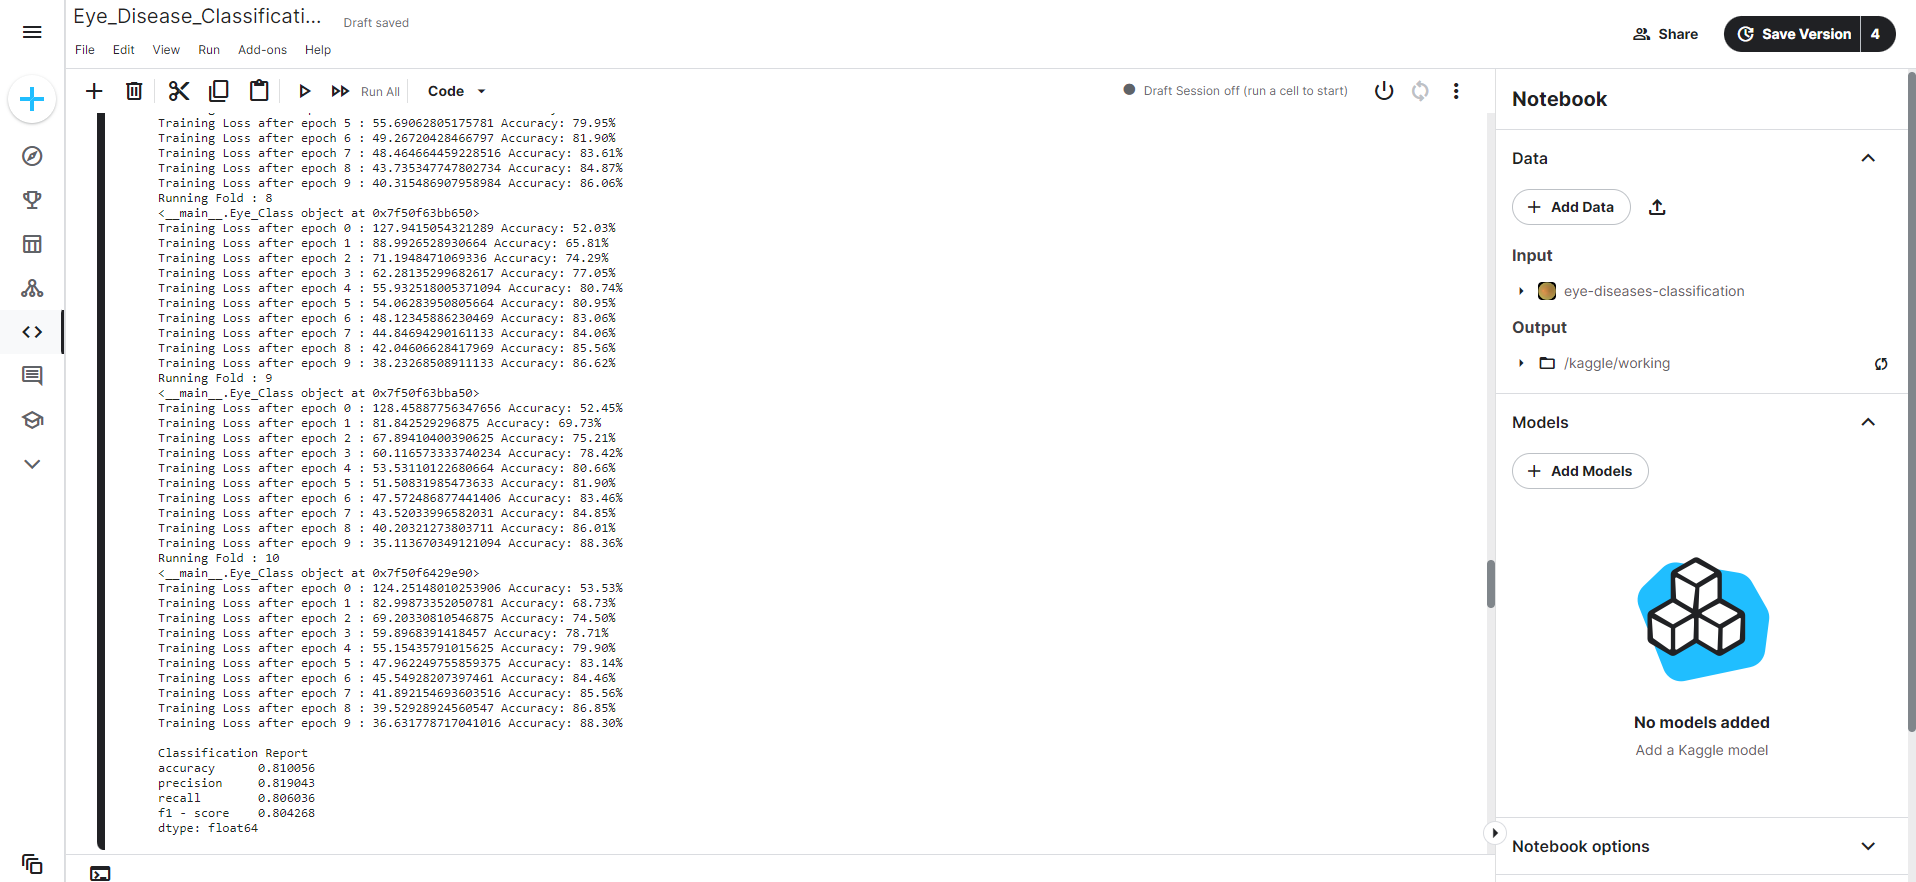
\includegraphics[width=\textwidth,height = 10cm]{Images/Kaggle Model Training.png}
    \caption{CNN Model Training}
    \label{CNN Model Training}
\end{figure*}

\section{Evaluation and Results}
\subsection{System Environment}
The model was trained locally on a mid-range system with the following specifications:
\begin{itemize}
  \item CPU: Intel i5 11 gen
  \item GPU: NVIDIA RTX 3050
  \item RAM: 16 GB memory
\end{itemize}

\vspace{5pt}
Additionally, We also used Kaggle IDE to train the model with the below specifications:
\begin{itemize}
  \item CPU Model: 79
  \item CPU Family: 6
  \item Model Name: Intel® Xeon® CPU @2.20 GHz
  \item CPU cores: 1
  \item Cache Alignment: 64
\end{itemize}

Training Deep learning models require considerable computing power. High performing GPU's have a parallel architecture which is rightly suited for deep learning. Using GPU's to train the models reduced the time considerably as parallel architecture of GPU's means faster computations simultaneously. Combining GPUs with cloud computing ensures significant reeducation in training times from weeks to hours for a deep leaning network.

\subsection{Hyperparameters}
The hyperparameters that we used to train our models are below:
\subsubsection{Batch Size - 32}
Batch size is the number of training examples used in one iteration of the training loop. Batch size is one of the most important hyperparameter as it signifies how many number of samples should be processed before updating the weights and biases so that our model makes better predictions in the next iteration. Our entire dataset is divided into batches, with each batch consisting of 32 samples. One of the advantages of having a smaller batch size is faster processing of the samples and less usage of memory.

\vspace{5pt}
\subsubsection{Optimizer - Adam}
Convolutional neural networks are trained using optimization algorithms. The main aim of this step is to repeatedly estimate the error for the current state using a loss function and then utilize that estimate to update the weights of the model. This reduces the mistakes that the model may make in the next iterations of the training.
\par
In this project, we have used Adaptive Moment Estimation (Adam) optimizer for our CNN. Adam is one of the most commonly used CNN optimizer and is much faster and efficient than the Stochastic Gradient Descent (SGD) which is the most basic optimizer for CNN's. Selecting the Right optimizer ensure that we extracting the most bit of accuracy from our CNN model.

\vspace{5pt}
\subsubsection{Loss Function - Cross Entropy}
A simple definition for a loss function is a method which evaluates how well our algorithm models our dataset. A loss function returns a loss value to indicate how close the predictions made by our model is to the original labels in the dataset. It outputs a higher loss value if the predicted class label probability is low for the actual target class label. Which means a low loss value indicates that our model is predicting well. Loss function plays a vital role in guiding the optimizers on how the weights should be updated to optimize the performance of the model.
\par
Cross Entropy calculates the score that summarizes the average difference between the actual and predicted probability distributions for all classes in the problem. The output of the probabilities ranges from 0 to 1 with 0 indicating a perfect cross-entropy value.

\vspace{5pt}
\subsubsection{Number of Folds - 10}
K-fold Cross validation is when a dataset is split or divided into K number of folds. For example if we say we have K=10 that means we have 10-fold cross validation. For our dataset we have used k as 10. K-fold cross validation ensures that variance of performance estimate is reduced and overfitting is avoided by training the model on different sets of randomized data.

\vspace{5pt}
\subsubsection{Number of Epochs - 10}
Epoch is the number of times our model iterates over the complete training set. One epoch processes all the batches through the model exactly once. Basically, it is equivalent to showing our model that whole training data bunch once. Our model accuracy increases as we train our model over multiple epochs. We have used 10 epochs for training our model Fig[\ref{CNN Model Training}].  

\subsection{Evaluation Criteria}
To check the correctness of the model and measure the quality we use Evaluation metrics. There are several metrics like Accuracy, Precision, Recall, F-1 Score and Confusion Matrix which we can use to evaluate our image processing model.

\vspace{5pt}
\subsubsection{Accuracy}
Accuracy is one of the most popular and reliable metric to evaluate the performance of our Image processing model due to its simplicity. Accuracy is defined as the total number of correct predictions made, divided by the total number of all predictions. However it is important to consider that accuracy might not be sufficient to evaluate the performance of CNN model, because of the type of dataset (symmetric vs non-symmetric) might affect. 

\vspace{10pt}
$Accuracy = \large\displaystyle\frac{TP + TN}{TP + FP + TN + FN}$
\vspace{10pt}

\begin{itemize}
  \item True Positive (TP): The number of positive instances that were correctly classified as positive.
  \item False Positive (FP): The number of negative instances that were incorrectly classified as positive.
  \item True Negative (TN): The number of negative instances that were correctly classified as negative.
  \item False Negative (FN): The number of positive instances that were incorrectly classified as negative.
\end{itemize}

\vspace{5pt}
\subsubsection{Precision}
Precision is defined as the ratio of true positive samples predicted versus the total number of positive samples predicted. Precision tells us how often the model is correct when it predicts a positive class.A high precision value is desirable in scenarios where the cost of false positives is high, for example in medical diagnosis, where a false positive can lead to unnecessary treatments and anxiety.

\vspace{10pt}
$Precision = \large\displaystyle\frac{TP}{TP + FP}$
\vspace{10pt}

\vspace{5pt}
\subsubsection{Recall}
Recall is defined as the ratio of correctly predicted positive samples to all available positive samples. Recall is a useful metric if we want to prioritize minimizing false negatives, meaning we want to avoid misclassifying true positives as negatives. For example, in a medical diagnostic task, it may be more important to identify all patients with a particular disease (true positives), even if some healthy individuals are falsely identified with the disease (false positives). In this case, recall would be a more important optimization metric  than precision.

\vspace{10pt}
$Recall = \large\displaystyle\frac{TP}{TP + FN}$
\vspace{10pt}

\vspace{5pt}
\subsubsection{F1 Score}
This metric is basically the weighted average of Precision and Recall I,e. it takes into account both false positives and false negatives for predicting the correctness of the model. Usually, the value of F1 score ranges from 0 to 1. A high score indicates that our model has a good performance, whereas the low score might indicates that our model has lot of false positives and false negatives. F1 scores are useful when we have an unbalanced data set where one class has significantly more occurrences than the other. In such a scenario,  high accuracy can be misleading, as the model may perform well in the majority class and poorly in the minority class. 

\vspace{10pt}
$F1 = \large\displaystyle\frac{2 * (Precision * Recall)}{Precision + Recall} 
$
\vspace{10pt}

\subsection{Cross-Validation}
Cross-validation is one of the most common techniques used in deep learning for evaluating the performance of the model. In Cross-Validation we divide the dataset into multiple subsets of data, and then we train and validate the model using these subsets of data. This process is then iterated over multiple times with different splitting of data, in order to train our model more efficiently.

\vspace{5pt}
One of the most popular forms of cross validation is K-fold cross-validation where the dataset is split into ‘k’ equally-sized folds Fig[\ref{K Fold Cross Validation}]. For example, if we use 10-Fold validation it means that in each iteration the dataset is split into 10 equally sized subsets. Then k-1 i,e. 9 folds are used for training the model and the remaining 1 fold is used for testing. The k-fold validation helps us remove any biases that may be present in our trained model and also helps us avoid the problem of overfitting. 

\begin{figure}[ht]
    \centering
    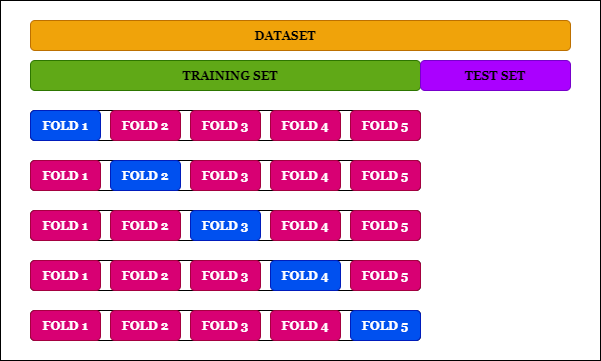
\includegraphics[width=8cm, height = 5.5cm]{Images/K Fold Cross Validation.png}
    \caption{K Fold Cross Validation}
    \label{K Fold Cross Validation}
\end{figure}

\vspace{5pt}
Also, k-fold validation provides a more accurate evaluation of model’s performance as compared to other methods such as holdout validation. This is because in k-fold validation the dataset is split multiple time as compared to holdout validation where the dataset is split only once. Overall k-fold does a better job in training the data more comprehensively over the data set in comparison to other methods.

\vspace{5pt}
Some of the limitations of using the k-fold cross validation as it may become computationally more expensive, if we choose a large value for K. For our model we have used k-fold validation with value of k as 10 ensuring that it does not require unfeasible computational power.

\subsection{Confusion-Matrix}
A confusion matrix is a performance evaluation technique that is commonly used in machine learning to assess the accuracy of a classification algorithm. It is a table Fig[\ref{Confusion Matrix}] that summarizes the predicted and actual classification results of a model on a set of data. The confusion matrix consists of four major components, True Positive, False Positive, True Negative and False Negative.

\begin{figure}[ht]
    \centering
    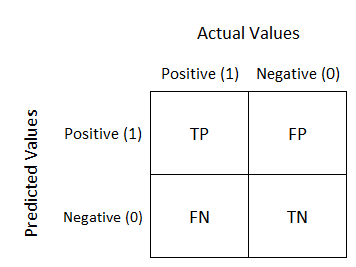
\includegraphics[width=8cm, height = 6cm]{Images/Confusion Matrix Example.png}
    \caption{Confusion Matrix}
    \label{Confusion Matrix}
\end{figure}

\vspace{5pt}
The rows of the matrix represent the actual (ground truth) class labels, while the columns represent the predicted class labels. The values in the cells of the matrix represent the number of instances that fall into each category.

\vspace{5pt}
A confusion matrix can be used to calculate several performance metrics of a classification model, such as accuracy, precision, recall, and F1-score. These metrics are computed based on the values in the cells of the matrix, and provide a more detailed understanding of the performance of the model. The confusion matrix is particularly useful when the classes are imbalanced, as it provides information about the distribution of errors in the classification task.

\subsection{Results}

\begin{figure}[ht]
    \centering
    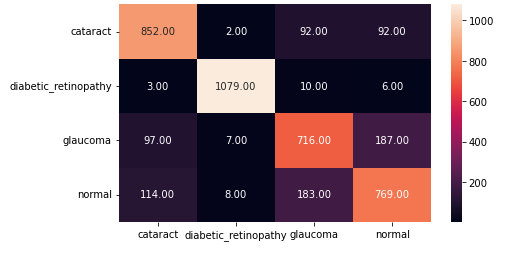
\includegraphics[width=9cm, height = 6cm]{Images/Confusion Matrix.png}
    \caption{Confusion Matrix of our Model}
    \label{Confusion Matrix of our Model}
\end{figure}

\vspace{5pt}
The Confusion Matrix provides a detailed breakdown of the model's performance in classifying the Image.From the matrix Fig[\ref{Confusion Matrix of our Model}], we can see that the model performed well in correctly predicting the normal category with 769 true positive predictions out of 1074 samples. But it struggled more with the cataract and glaucoma classes, with 92 and 187 false negative predictions, respectively. The model had greater accuracy in correctly predicting diabetic retinopathy with 1,079 true positive predictions out of 1,098 samples.


\begin{figure*}[ht]
    \centering
    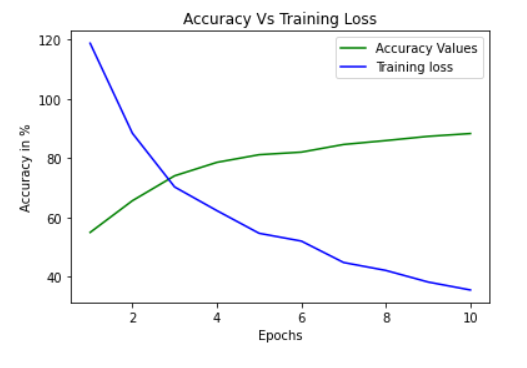
\includegraphics[width=0.9\textwidth,height = 10cm]{Images/Accuracy Vs Training Loss.png}
    \caption{Accuracy Vs Training Loss}
    \label{fig:Accuracy Vs Training Loss}
\end{figure*}


\vspace{5pt}
In this project, K-Fold cross-validation was used to evaluate the performance of the models. The accuracy and training loss were plotted Fig[\ref{fig:Accuracy Vs Training Loss}] to understand how they vary across epochs within each fold. These metrics correspond to the loss and predictions that are used for back propagation during training. Across all models, there were consistent and uniform metrics observed across folds. This indicates that the model is robust and stable across different training instances and is not overfitting to the training data.

\vspace{5pt}
\begin{table}[h]
\centering
\begin{adjustbox}{width= 5cm, height=1.5cm}
\begin{tabular}{|c|c|}
\hline
\textbf{Metrics} & \textbf{Value} \\ \hline
Accuracy & 0.810056 \\ \hline
Precision & 0.819043 \\ \hline
Recall & 0.806036 \\ \hline
F1-score & 0.804268 \\ \hline
\end{tabular}
\end{adjustbox}
\vspace{5pt}
\caption{Classification report}
\label{tab:Classification report}
\end{table}

\vspace{5pt}
The table [\ref{tab:Classification report}] shows the performance metrics of the image classification model that achieved an overall accuracy of 0.8136 on the test dataset. The model has an accuracy of 0.8207, indicating that the majority of images that the model classifies as positive are actually positive. The recall of the model is 0.8102. This means that the model correctly identified most of the positive images in the dataset. The model's F1 score, which is the harmonic mean of precision and recall, is 0.8094, representing an overall balance between precision and recall. These results indicate that the model achieved a good level of accuracy and reliability in classifying images. However, these metrics do not provide a complete picture of model performance and further analysis may be required to assess suitability for a particular application. For Example, additional metrics like specificity and AUC-ROC curve may have to be evaluated for better understanding about the model's performance across different classification thresholds.

\begin{figure}[H]
    \centering
    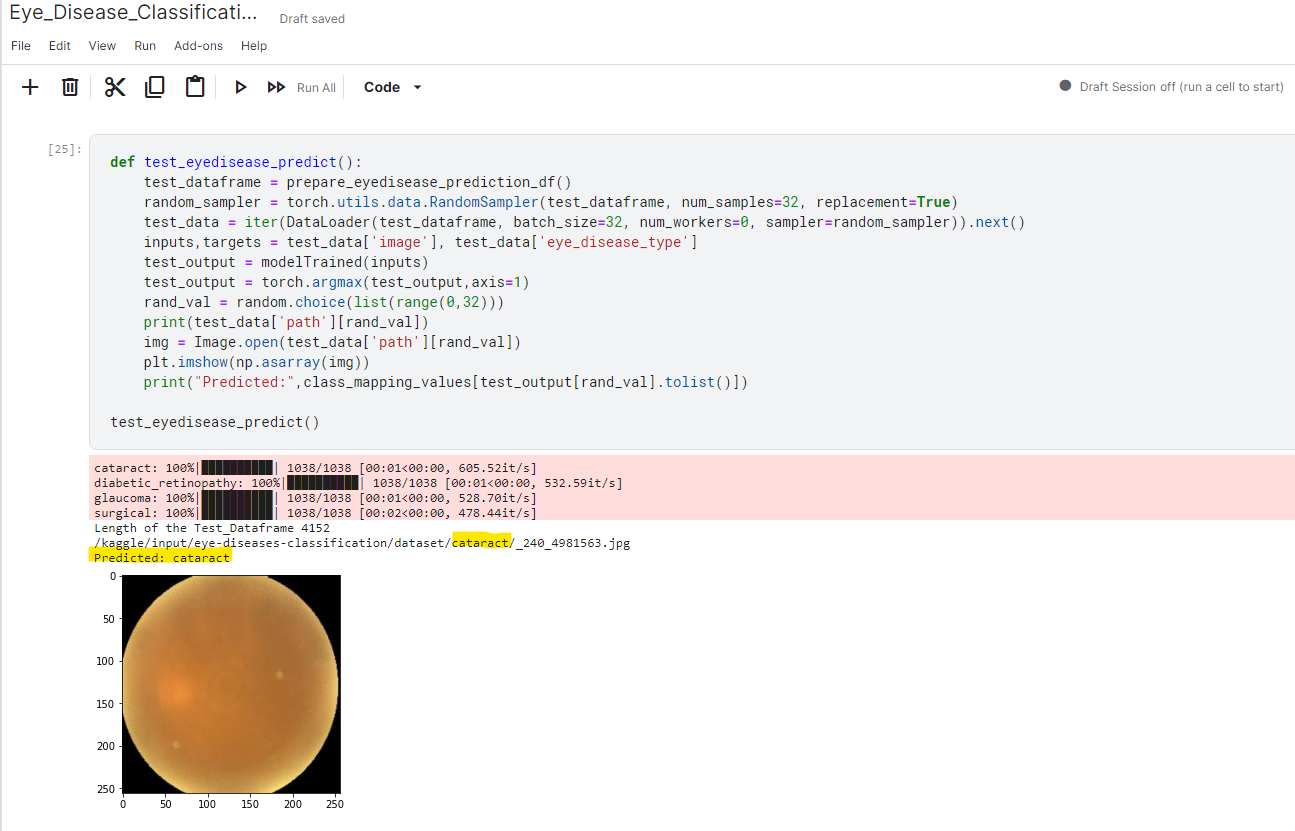
\includegraphics[width=9cm, height=7cm]{Images/Test Image.png}
    \caption{Sample Disease Prediction}
    \label{fig:Sample Disease Prediction}
\end{figure}


\vspace{5pt}
With the developed CNN deep learning model, we predicted the output of a image from the test set Fig[\ref{fig:Sample Disease Prediction}]. The prediction result showed that the model was able to accurately classify the input image into one of the eye disease categories with high confidence. This demonstrates the effectiveness of the developed CNN model in classifying retinal images and detecting eye diseases.

\vspace{5pt}
\section{Conclusion and Future Work}
In this study we proposed an approach which used deep learning technique based on CNN architecture for early detection of eye diseases like diabetic retinopathy, cataract and glaucoma. The model was trained and its performance was evaluated based on various metrics. Overall, our results from this study indicates that CNN-based model has the potential to accurately predict and classify eye related diseases in a timely manner. These types of models can be a cost effective, reliable and time efficient alternative to traditional diagnostic methods. Also, this technology has the potential to significantly reduce the burden on healthcare professionals and in ensuring timely detection and treatment of eye related diseases for patients

\vspace{5pt}
We can further improve model architecture by implementing more advanced CNN architectures like DenseNet and ResNet. We can further train our model on larger dataset to ensure that evaluation metrics improve. Also, in future we can develop web and mobile based application based on our CNN model which helps user check for these diseases in their eye by taking photos through there smartphone camera. This will ensure that patients can easily access such technology with the help of internet and eliminating the need for a doctor to diagnose the same.

\begin{thebibliography}{00}
\bibitem{b7} M. D. Abràmoff, J. C. Folk, D. P. Han, et al., "Automated Analysis of Retinal Images for Detection of Referable Diabetic Retinopathy," IEEE Transactions on Medical Imaging, vol. 29, no. 1, pp. 136-154, Jan. 2010.

\vspace{5pt}
\bibitem{b8} Oluwatobi Noah Akande, Oluwakemi Christiana Abikoye, Aderonke Anthonia Kayode, Yema Lamari, "Implementation of a Framework for Healthy and Diabetic Retinopathy Retinal Image Recognition", Scientifica, vol. 2020, Article ID 4972527, 14 pages, 2020. \url{https://doi.org/10.1155/2020/4972527}

\vspace{5pt}
\bibitem{b9} Sarki, R., Ahmed, K., Wang, H. et al. Image Preprocessing in Classification and Identification of Diabetic Eye Diseases. Data Sci. Eng. 6, 455–471 (2021). \url{https://doi.org/10.1007/s41019-021-00167-z}

\vspace{5pt}
\bibitem{b10} F. Alzami, Abdussalam, R. A. Megantara, A. Z. Fanani and Purwanto, "Diabetic Retinopathy Grade Classification based on Fractal Analysis and Random Forest," 2019 International Seminar on Application for Technology of Information and Communication (iSemantic), Semarang, Indonesia, 2019, pp. 272-276, doi: 10.1109/ISEMANTIC.2019.8884217.

\vspace{5pt}
\bibitem{b11} Kumar, Y., Gupta, S. Deep Transfer Learning Approaches to Predict Glaucoma, Cataract, Choroidal Neovascularization, Diabetic Macular Edema, DRUSEN and Healthy Eyes: An Experimental Review. Arch Computat Methods Eng 30, 521–541 (2023). \url{https://doi.org/10.1007/s11831-022-09807-7} 

\vspace{5pt}
\bibitem{b12}
U. R. Acharya, N. Kannathal, E. Y. K. Ng, L. C. Min and J. S. Suri, "Computer-Based Classification of Eye Diseases," 2006 International Conference of the IEEE Engineering in Medicine and Biology Society, New York, NY, USA, 2006, pp. 6121-6124, doi: 10.1109/IEMBS.2006.260211.

\vspace{5pt}
\bibitem{b13}
M. R. Ahmed , S. R. Ahmed , A. D. Duru , O. N. Uçan and O. Bayat , "An Expert System to Predict Eye Disorder Using Deep Convolutional Neural Network", Academic Platform - Journal of Engineering and Science, vol. 9, no. 1, pp. 47-52, Jan. 2021, doi:10.21541/apjes.741194

\vspace{5pt}
\bibitem{b14} M. Jena, S. P. Mishra and D. Mishra, "Detection of Diabetic Retinopathy Images Using a Fully Convolutional Neural Network," 2018 2nd International Conference on Data Science and Business Analytics (ICDSBA), Changsha, China, 2018, pp. 523-527, doi: 10.1109/ICDSBA.2018.00103.

\vspace{5pt}
\bibitem{b15} Eye Disease Retinal Images, en.[Online] Available : \url{https://www.kaggle.com/datasets/gunavenkatdoddi/eye-diseases-classification}


\end{thebibliography}

\end{document}

